
\chapter{Proposed Indexing Model}

Before we integrate machine learning models on conventional spatial data indexes, we should review the current state-of-art learned indexes and spatial indexes. The most important idea that comes from the learned indexes is to use learned models to predict the possible location of the key. In RMI, a query point is passed into a sequence of learned models to get the final range of location. ALEX improved on RMI using a \textit{Gapped Array} or a \textit{Packed Array} to store data points, instead of searching in a single array. The RMI is more memory efficient compared to ALEX since all the data points are allocated in a contiguous array, whereas ALEX allocates data points at a different location in memory. The PGM-index uses piecewise linear models to create segments of linear models. The number of segments controls the trade-off between time and space. 

We must concede that the learned models can not predict the exact position, there always are errors that come with the predicted value. Reducing the error will rely on more complex computations, but inference cost will also be expensive. The question is how many trade-offs we can afford to build either a time-efficient spatial index or space-efficient spatial index. 

Difficulties of spatial data is the consistency of simultaneity ordered on different dimensions. The ZM’s approach is to combine the Z-order space-filling curve and the RMI model, but it does not guarantee to find data points accurately and it does not support k nearest neighbour query.  The RSMI also adopted Z-order curves to apply to spatial space partitioning. The structure of the RSMI is also similar to the RMI and the R-Tree, because of the recursive model and space partitioning. 

Current learned spatial indexes have a complex hierarchical structure. The hierarchical structure allows the index to handle complex spatial queries. The problem with adopting learned models to the hierarchical structure is the prediction value can have a large error range. The error propagation can be solved by introducing a sub-model to refine search regions. However, it can still cause problems when handling skewed data and error bounds are large. A large error bound can produce overhead on the number of access of sub-trees. As a result, it can degrade query performance. 

\section{Design Goal}

Before investigating methods to build an efficient spatial index, the design goal of the learned spatial index meet the following requirements:
\begin{itemize}
    \item The spatial index must retrieve query points \textbf{accurately}. 
    \item The spatial index can handle \textbf{Point Match Query}, \textbf{Range Query} and the \textbf{Nearest Neighbour Query}.
    \item The data distribution should be mapped by a \textbf{cumulative distribution function} (CDF). 
\end{itemize}


Firstly, retrieving the query point is the most important function in the spatial index. The Point Match Query is defined in \ref{def:pmq}, it retrieves a data point from the index for a given pair of coordinates. Therefore, accurate point retrieval is a basic and important function of a spatial index. Secondly, one of the major differences between a one-dimensional index and a spatial index is that a spatial index is able to handle spatial specific queries. The Point Match Query is the foundation query for supporting various spatial queries.


\textbf{Efficiency} is also an important criterion for measuring the performance of a spatial index. As mentioned above, it is hard to balance the trade-off between time and space. The ideal scenario is to achieve a fast query time with a low memory cost for a spatial index. However, in reality, we sometimes have to sacrifice one for another. The designed spatial index should exploit the space-time trade-off, and try to optimize from at least one aspect. 

Overall, we are focusing on two aspects when designing a spatial index: query result accuracy, complete functionality of spatial query and performance improvement. The following sections describe how a \textit{Learned Hashmap} can be useful in a spatial index and achieve these goals. 


\section{The Learned Hashmap}

\subsection{Overview}
\begin{figure}[ht]
\centering{
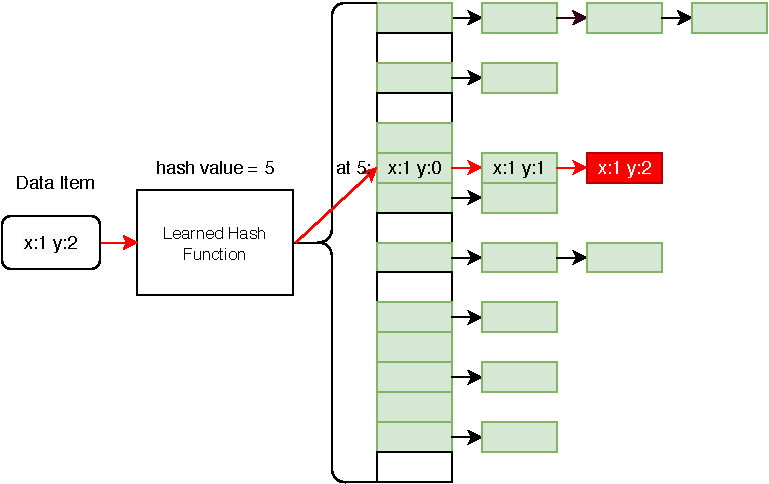
\includegraphics{Figures/hashmap.pdf}
\caption{The structure of the Learned Spatial Hashmap(LSPH). The search flow in LSPH takes one value from the selected dimension, then the learned hash function predicts the index to the estimated location in the hashmap.}
\label{fig:learned_spatial_hashmap}
}
\end{figure}

The Learned Spatial Hashmap(LSPH) is an efficient learned data index method for storing spatial data and handling spatial queries. The structure of the LSPH is straightforward, the main component of the index is a learned hashmap with chaining, as shown in Figure \ref{fig:learned_spatial_hashmap}. The learned hashmap is a hashmap with a learned CDF as its hash function \cite{Kraska:2017vh}. The CDF learned from a machine learning model and used it as a hash function in the hashmap. Linked lists are used in the LSPH for chaining. The design of the LSPH building process makes it suitable for storing spatial data points. The build process of the LSPH is shown as follows:

\begin{enumerate}
    \item \textbf{Dimension Selection}: Choosing one dimension from the dataset for model training.
    \item \textbf{Model Training}: A learned model trains on the selected dimension of data. 
    \item \textbf{Building of the LSPH}: Creating and Inserting to the Hashmap based on the prediction value.
\end{enumerate}

The learned model in LSPH trained only on a single dimension of two-dimensional data points. We select a single dimension of value from a coordinate data pair: $\{n|\forall n \in E.p\}$, where $E$ is every element in the dataset, and $p$ is selected dimension. The dimension selection is based on the  divergent of the values. A more divergent set of values can produce more divergent prediction values  from the same model. Therefore, it will optimize the loading factor of the hashmap, thus improving the efficiency of the lookup speed.

Using simple linear regression to train on data along a selected dimension $p$, with corresponding ranks of the data points, we can estimate a range of candidate positions of the query data point on the $p$ dimension, and trained model $m$. 

Memory with a size of the model prediction range will be allocated in the hashmap: $\hat{y}_{max} - \hat{y}_{min}$. The building process of the hashmap is relatively simple, the trained model $m$ inferences the input values from the same selected dimension $p$. Then the trained model yields a prediction value that can be treated as the hash value for the hashmap. Finally, the data point can be inserted into the hashmap at the index of the hash value. 

The LSPH is similar to a regular hashmap. It is simple but yet powerful. Some major differences distinguish itself from a regular hashmap, and suitable for storing and searching spatial objects. The LSPH uses only values from one dimension for the entire building procedure. Some properties about the learned hashmap guarantee the performance and accuracy of querying results, it will be discussed in the Section \ref{the_learned_hashmap}. 


\subsection{Single Dimensional Index Building}


\begin{figure}[ht]
\centering
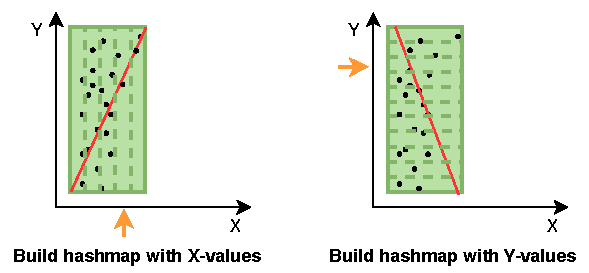
\includegraphics{Figures/single_dimension.pdf}
\caption{Difference between building data with x-values and y-values}
\label{fig:single_dimension}
\end{figure}

In the LSPH, the building process and the initial search range relies on one dimension of data. It is much easier to handle one-dimensional data than multidimensional data. The selection of the dimension for training is determined by the variance. Values on which dimension with a larger variance will be selected for model training. Given a series of two dimensional data $S = (x_i,\, y_i)$, compare the variance between $Var(x) \, \forall \, x \subseteq S$ and $Var(y) \, \forall \, y \subseteq S$, and dimension $p$ selected by the greater value between these two variances.


Transformation(space-filling curves, endpoint transformation and midpoint transformation) tends to be a popular choice for transferring multidimensional data into one-dimensional data in many traditional spatial indexes. In spatial data, it is hard to map two-dimensional data into one-dimensional data while preserving the spatial proximity \cite{Gaede:1998fp}. The space-filling curves (SFC) integrate both x-value and y-value into one value, to preserve the locality of points in the space. The calculated SFC values are used to rank the data points. Two closely-ranked data points in sorted order are also located close to each other in the spatial space. However, it requires extra calculations, and more importantly, a learned model can not produce an accurate prediction for the SFC values. 


There are some benefits for a spatial index to indexing from a single dimension of data. Training on a single dimension of values preserves the original information about the location, and it is already a one-dimensional data available. As a result, the LSPH has a fast query performance, since there is no pre-calculation for the transformation, values from original data can be used directly for inference. The building performance is also fast because of no extra calculation during the building process. 

Training on only a single dimension might also avoid potential data skewness. In most spatial datasets, skewness is most likely to happen in only one dimension. It means if one dimension is skewed, we can check if another dimension is skewed, and the training dimension $p$ is chosen from the less skewed out of two. Although there are some special cases, which values in both dimensions are skewed (such as two clusters of data points). It only creates computation overhead during searching in the chaining, and will not affect the accuracy of query results. 

 The selection of $p$ dimension can affect the space utility in the LSPH. A load factor in a hashmap is defined as: $\textit{Load Factor} = \frac{\textit{n}}{\textit{k}} $, where $n$ is \textit{number of entries occupied in the hashmap} and $k$ is \textit{size of hashmap}. Performance of the hashmap is largely decided by the load factor \cite{hashmap}. For example, a hashmap with a load factor of $0.5$ represents only half of the slots in the hashmap that are loaded with values. The hashmap in the LSPH is created with a size of prediction range, so in general, a high load factor can reduce chaining overhead and increase space utilization. 


\subsection{Learning a Hashmap} \label{the_learned_hashmap}


The learned hashmap has been mentioned in Kraska’s paper \cite{Kafle:2017dy}. He suggested that the learned hash map is no better than traditional hashmaps such as Cuckoo hashing in terms of solving conflict and distributing key mapping. There are some properties of the learned hashmap not mentioned in Kraska's paper, which can be strengths for handling spatial query operations. 


\textbf{Small hash collision rate}: According to Kraska, the learned hashmap can reduce hash conflict by up to 77\%. The logic behind it is that a randomized hash function is a trend to generate a random hash value, whereas the learned CDF can produce a hash value that grows with an increase of the input value. Therefore, it is less likely to have hash collisions with learned hash functions.

\textbf{Sorted head nodes}: Since the prediction results monotonically grow with the input value, the order of head nodes in the learned hashmap is sorted. In a set of sorted data, for any values $x\prime$ that are greater than a given input value $x$, the predicted value from the learned CDF function $y\prime = \text{CDF}(x\prime)$ is also greater than the predicted value $y = \text{CDF}(x)$. Kristo \cite{Kristo:2020it} implemented a sorting algorithm based on this property of the learned hashmap. 


\textbf{Load factor depends on model and data distribution}: The trained CDF maps all values from the dataset to the index value in the hashmap. Therefore, a good model choice and also the distribution of the data can affect the load factor. Whereas, the load factor in a hashmap that uses a random hash function is predetermined. This is critical to both memory space efficiency and query time performance. A high load factor can reduce the length of chaining to utilize the existing memory space in the hashmap, and also reduce the lookup overhead in the chaining. 

\textbf{Cost of hash function depends on the model}: Query performance also depends on the complexity of the learned model. In general, we want to have a model that can map the approximate distribution of data. However, if the model is complicated, then the query performance at inference can be affected. Rather, a high load factor in the hashmap is more important than having a computationally more expansive model for the query performance. 

\textbf{Guarantee to find value(completeness)}: Most learned indexes are attempting to search the position of the value key directly, but the prediction value always comes with an error bound. The model in LSPH does not predict the position of the index directly but is used as a hash value to access the position in the hashmap and potential chaining at that location. Therefore, the LSPH can guarantee to find the position of the key or the chaining where the key belongs to with one shot. 


Overall, these properties provide a foundation for the LSPH. The structure of the hashmap, monotonicity of head node and small collision rate are crucial for query accuracy, query performance and implementing spatial query algorithms. Compared to other learned indexes, the accuracy of a point query relies on the structure of the hashmap, rather than model prediction. Hence, the LSPH can guarantee the search result accuracy. 

\subsection{Model for Learning}
The query performance is largely dependent on the model and the distribution of data. Because the prediction value is used as a hash value instead of the actual position of the key in the hashmap, the model does not need to be well fitted with the dataset. Neural networks are better for fitting data well, but it also takes a long time for training, and more expensive at inference. A linear model can do a good job, because the computation is much simpler. With a trained weight $w$ and bias $b$, linear function $y = wx \dot b$ can map an approximate distribution of data, and it can achieve a good performance at inference. Therefore, linear regression is chosen as the learned model for the LSPH, and the least square method is used for training the two parameters. As a result, the building process of LSPH is also fast. 


\section{Update Handling}
The basic operations including insert, delete and update in the LSPH are also almost identical to a regular hashmap. Rather than changing the way a hashmap is used, we changed the data item content and made it suitable for handling spatial objects. Points in spatial space usually contain the coordinates of its location, which is ${x, y}$. As mentioned above, a dimension $p$ is chosen for model training, and it is also used for all operations of the LSPH. 


\begin{figure}[ht]
\centering
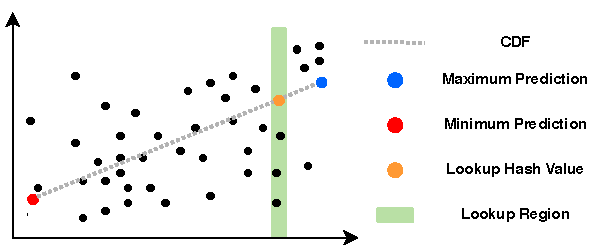
\includegraphics{Figures/search.pdf}
\caption{Lookup process on the dataset. Using the trained linear regression model to calculate the lookup hash value, then scanning the lookup region base on the lookup hash value.}
\label{fig:search}
\end{figure}


\textbf{Search}: Insertion and deletion heavily rely on searching data items in a data index. Searching an item in the LSPH requires hashing and chaining. $x-value$ or $y-value$ is chosen for hashing, based on the chosen $p$. A hash value is generated by the prediction value from the learned model: $h : V \rightarrow H$, where $H: \Leftrightarrow CDF$. The size of the LSPH is determined by the maximum and minimum prediction values: $m = \hat{y}_{max} - \hat{y}_{min}$, so when searching in the LSPH, the prediction value must subtract the minimum prediction value among the entire dataset to fit in the hashmap. The default rounding method to rounding from the float prediction value to integer is floor rounding. We found that rounding the closest integer can increase the variability of the resulting hash values, and raise the load factor. 


\textbf{Separate Chaining}: When a slot is occupied in the hashmap, the hash collision happens. A linked list will be created for chaining to solve the hash collision, any items that collided at the index in the hashmap will be appended to the end of the linked list. The length of the chaining is also determined by the load factor of the hashmap. Since the size of the hashmap is corresponding to the range of all prediction values, the higher the load factor is, the shorter the chaining will be. 

\textbf{Update}: To update an item, we need to determine whether the hash value of the data item is within the hashmap size of $m$. If the hash value is within the range, then we can insert the item as usual. If it is out of the range, the hashmap needs to be updated. The hash function model will be recalculated, and all existing items will be rehashed from the updated model. Since the linear model is used and the insertion process is relatively fast compared to neural network training, the rehash process is not considered expensive. 

\section{Query Processing}
The structure of LSPH adopted from the learned hashmap. What makes it able to manage spatial data is spatial query algorithms. Three types of spatial queries that are currently supported by LSPH: \textit{Point Query}, \textit{Range Query}, and \textit{k Nearest Neighbour query}. These three queries are focused on point object handling, but also developed a bounding box query algorithm that supports more complex spatial objects other than point objects.  

The most important and frequently executed operation is lookup a key. Key lookup in LSPH requires a hashing and iterative searching in the separate chaining. The performance of the lookup query is bounded by the length of chaining since the cost of hashing and indexing is always $O(1)$. The total cost of searching in the LSPH is $O(1 + \frac{n}{k})$, , where $\frac{n}{k}$ is the load factor. 

\subsection{Point Query}
\begin{algorithm}[H] \label{point_query}
\SetAlgoLined
\KwIn{Query point $q \ni {x_q, y_q}$}
\KwOut{Result query point $q_result$ that stored in the structure}
 $x\leftarrow{x_q}$, $y\leftarrow{y_q}$\;
 hashKey $\leftarrow{\text{hashFunc}(sort\_by\_x ? x : y)}$\;
 tempNode $\leftarrow{\text{table[hashkey]}}$\;
 \While{tempNode is not empty}{
  \eIf{tempNode.y $=$ y}{
    \If{tempNode.x $=$ x}
        {return tempNode\;}
   }{
   tempNode $\leftarrow{getNext()}$\;
  }
 }
 return null\;
 \caption{Point Query}
\end{algorithm}

The procedure of spatial point lookup consists of two parts: 
\begin{enumerate*}
    \item single dimensional value hashing
    \item local search in chaining.
\end{enumerate*}
 The steps are defined in Algorithm \ref{point_query}.

As described in previous sections, LSPH training used values on only one dimension. Therefore, a boolean variable $sort_by_x$, which is deducted from the single-dimensional index building,  is determining which dimension $p$ will be used in point lookup. Next, the selected value of $x$ will be hashed from a learned model. Since a linear model is mapping the approximate shape of the distribution of the dataset, the prediction/hash function is 
\begin{equation}
\hat{y} = x * w + b + 0.5f - (x<0)
\end{equation}
, where $0.5f - (x<0)$ is rounding float numbers to the closest integer value including negative numbers. Finally, a local iterative search is to find the actual position of the target tuple of spatial points, by comparing the value from another dimension and validate the selected value on $p$ dimension. 

The performance of the \textit{Point Query} is great for a uniformly distributed dataset since the querying process only requires one multiplication, one addition and local iteration with a size of  $\frac{n}{k}$. For all keys that share the same hash value will be placed in the same chaining. Therefore, the LSPH will guarantee to find the point. 


\subsection{Range Query}

\begin{figure}[ht]
\centering
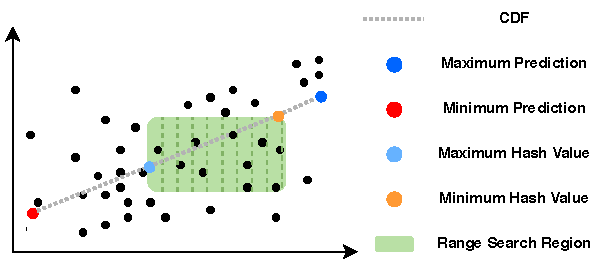
\includegraphics{Figures/range_search.pdf}
\caption{\textit{Range Query} in LSPH. Calculate the maximum and minimum hash value to get the search region on the hashmap.}
\label{fig:range_search}
\end{figure}


\begin{algorithm}[H] \label{range_query}
\SetAlgoLined
\KwIn{Range of search window $r$}
\KwOut{Set of result points $S$}
 $xMin, xMax, yMin, yMax\leftarrow{r}$\;
 $hashKeyMin = \text{hashFunc}(sort\_by\_x ? xMin : yMin)$\;
 $hashKeyMax = \text{hashFunc}(sort\_by\_x ? xMax : yMax)$\;
 $S\leftarrow{\emptyset}$\;
 \For{hashkey in from hashKeyMin to hashKeyMax}
 {
 tempNode $\leftarrow{\text{table[hashkey]}}$\;
    \While{tempNode is not empty}{
        \If{tempNode.x in $r$}
        {
            append tempNode to $S$\;
        }
        tempNode $\leftarrow{getNext()}$\;
    }
 }
 
 return $S$\;
 \caption{Range Query}
\end{algorithm}


\textit{Range Query}, in addition to \textit{Point Query}, requires to specify the search range and scan through every data item if qualified. As illustrated in Figure \ref{fig:range_search}, first to find the $hashKeyMin$ and $hashKeyMax$ for the minimum and maximum x value, or minimum and maximum y value, depending on the $sort_by_x$. Then we can scan through every chain within the search region in the hashmap, to check if a data item from a node is in the searching range.

One of the properties of the monotonic growing learned map is that the values in the head nodes are sorted. Therefore, the $hashKeyMin$ and $hashKeyMax$ is defining the bounds of the search region. Any index value on the hashmap that exceeds the $hashKeyMin$ and $hashKeyMax$ will be out of the target region. At each chaining bucket, it just needs to check if points are within the range and if true then append the point to the result list. The time complexity for the range query depends on the size of the search region and the length of chaining.  



\subsection{k Nearest Neighbours Query}

\begin{figure}[ht]
\centering
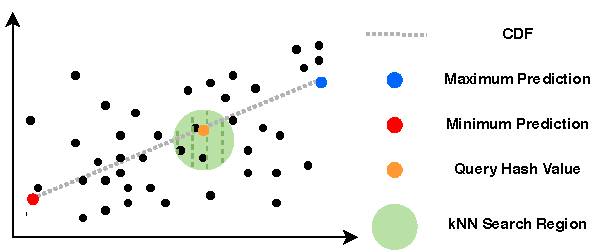
\includegraphics{Figures/knn.pdf}
\caption{\textit{kNN Query} in LSPH. First to calculate the query hash value, then expand to neighbour buckets.}
\label{fig:knn}
\end{figure}



\begin{algorithm}[H] \label{knn_query}
\SetAlgoLined
\SetKwProg{Def}{def}{:}{}
\KwIn{Query point $q$; Number of nearest neighbours $k$}
\KwOut{Set of result points $S$}
$x\leftarrow{x_q}$, $y\leftarrow{y_q}$\;
hashKey $\leftarrow{\text{hashFunc}(sort\_by\_x ? x : y)}$\;
S $\leftarrow$ Priority Queue\;


% \tcp{Searching at current position in the table[hashKey]}

\Def{localSearch(hashKey)}{
    tempNode $\leftarrow{\text{table[hashKey]}}$\;
    \While{tempNode is not empty}{
        \If{$dist(tempNode, q) \leq minDist$}
            {append tempNode to S}
        tempNode $\leftarrow{getNext()}$\;
    }
}
% \tcp{ Search in current index is finished, starting search at expanding index in the table}

i $\leftarrow{hashKey+1}$; 
j $\leftarrow{hashKey-1}$\; 
previousMaxDist $\leftarrow{\text{S.Max()}}$;
localMinDist $\leftarrow{0}$\;
\While{localMinDist $<$ previousMaxDist}
 {
    previousMaxDist $\leftarrow$ previous S.Max()\;
    localSearch(i); localSearch(j)\;
    localMinDist $\leftarrow$ S.Min()\;
    i++; j--\,--\;
 }
 
 
 return $S$ with first k elements\;
 \caption{k Nearest Neighbours Query}
\end{algorithm}

The \textit{k Nearest Neighbours Query} finds $k$ number of point neighbours that have the closest distance to query point $q$. The algorithm starts with the same hashing process as in \textit{Point Query} and \textit{Range Query}. It first compares the distances with the current bucket of chaining, and stores the candidate into a priority queue that prioritizes based on the closest distance. Once it has been explored at the current index, it can expand the exploration to neighbour indexes. Since the indexes are sorted based on the monotonic growth of head nodes, the neighbour indexes are containing the closest nodes to the query node. Hence, the next step of the searching process will use two pointers, which one is doing an incremental search, and another one is doing a decremental search along the hashmap. The expansion search process will stop until the minimum of distances that collected at the current index is greater than or equal to the maximum distances collected previously.  Finally, k items pop out of the queue and return as the result of k nearest neighbours search

The time complexity of Algorithm \ref{knn_query} is $O(1 + m\frac{n}{k})$, where $m$ is the size of expansion. Unlike hieratical structures such as B-Tree, the linear structure allows reducing redundant data scans caused by overlapping regions. Hence, LSPH can achieve more efficient kNN searching by fast hash computation and scanning regions reduction. 

\section{Bounding Box Handling}

\begin{figure}[ht]
\centering
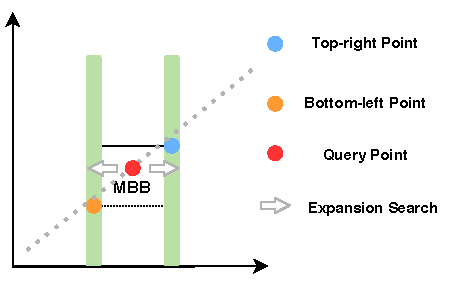
\includegraphics{Figures/object.pdf}
\caption{Store the top-right and bottom-right corners of a MBB in the hashmap}
\label{fig:object}
\end{figure}

The current process discussed above is all based on the point object in spatial data. We also implemented a method that allows the spatial index to handle more complex spatial objects such as line segments and polygons. All two-dimensional objects can be bounded by their minimum bounding box (MBB), which is a rectangle shape box defined by the minimum and maximum width and height of the object. The representation of MBB simplifies the structure of spatial objects. The $x$ and $y$ coordinate of two diagonal corner pointers are taken to store MBB in the LSPH.  

The fundamental operation of MBB supported by the LSPH is for a given query point $q$, the search result returns the MBB that the $q$ belongs to. To check if a point is within a particular MBB, both of the corner points need to be compared with the query point. Therefore, we have to insert both of the corner points of the same MBB into the LSPH. Each data item contains the $x$ and $y$ coordinate of the corresponding corner, and a pointer to extra information of the data item that contains coordinates from both corners. 

To retrieve the MBB from the query point, the procedure is similar to the k Nearest Neighbours Query: 
\begin{enumerate}
    \item Calculate the hash value from query point $q$.
    \item Search at the current index, which is the hash value.
    \item Iterative searching in the linked list at the current index. 
    \begin{enumerate}
        \item Retrieve coordinates of two corner pointers from data items in the linked list. 
        \item Check if the query point is within the currently searching MBB (defined by the two corner coordinates).
        \item If it is within the MBB region, return that MBB.  
    \end{enumerate}
    \item If no MBB found at the current index, expand the index to both sides (add and subtract the pointer). Repeat the search process.
\end{enumerate}

The performance of MBB searching is also similar to the performance of kNN query, except that MBB does not require a $k$ number of return values. Since we insert both the lower-left corner and upper-right corner into the hashmap, the searching pointer can compare to either corner arbitrarily. A pointer stores coordinate values of both corners are pointing to the hashmap item, so no matter which corner that the current searching pointer is comparing with, it can access the full information of both corners. 

There is one issue that can occur when two MBBs are overlapping, but the polygons themself do not overlap, the result will only return the first found MBB. To find the finer search result over polygon spatial objects, the information of the shape of the polygon is needed to calculate if the search point is within the polygon. 

\section{Summary}
